\section{Računalni vid}
Računlani vid je veliko područje umjetne inteligencije koje se bavi algoritmima i metodama vezanim za obradu slike. Računalni vid podjeljen je u nekoliko podkategorija:
\begin{enumerate}
\item \textbf{Klasifikacija i Lokalizacija.} Ovo područje računalnog vida bavi se prepoznavanjem objekata na slici. To znači da algoritam odlučuje kojem razredu (\textit{engl.} class) pripada cijela slika. Pretpostavljajući navedeno, lokalizacija je proces pronalaženja pozicije objekta na slici. Rezultat procesa lokalizacije obično je crtanje okvira (\textit{engl.} bounding box) oko objekta na slici. Pobjednici natjecanja "Large Scale Visual Recognition Challenge 2017 (ILSVRC2017)" u kategoriji klasifikacije pobijedili su sa rezultatom od 2.251\% pogreške, dok su pobjednici u kategoriji lokalizacije postigli rezultat sa greškom od 6.226\%. Sa slike \ref{img:ILSVRC} vidi se da su se razultati u odnosu na 2016. godinu popravili za 0.8\% u kategoriji klasifikacije te 1.5\% u kategoriji lokalizacije .
\begin{figure}[htb]
\centering
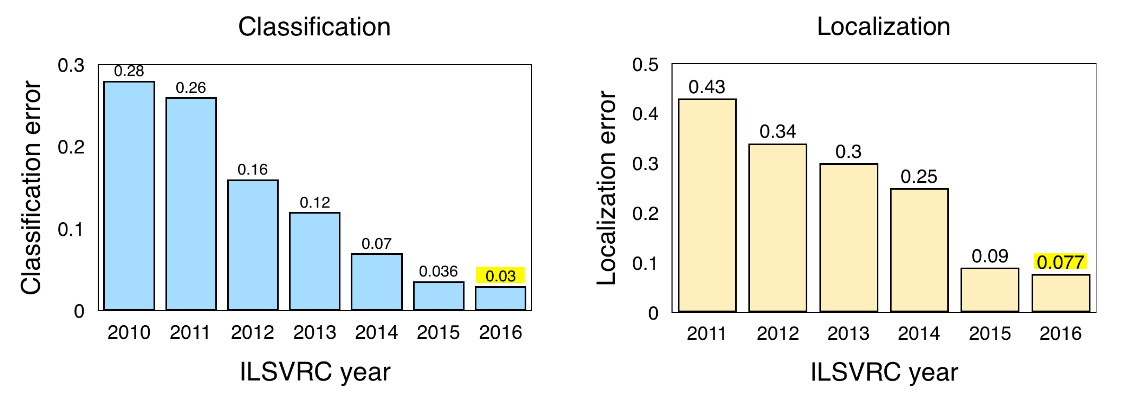
\includegraphics[width=\linewidth]{img/ILSVRC.png}
\caption{Rezultati natjecanja ILSVRC tokom godina \citep{ILSVRC}}
\label{img:ILSVRC}
\end{figure}

\item \textbf{Detekcija.} Pod pojmom detekcija podrazumijeva se pronalaženje objekata na slici, odnosno, određivanje prisutnosti objekata na slici. Proces detekcije objekata je malo složeniji od kalsifikaije/lokalizacije objekata zbog toga što se ovdje mora provesti više klasifikacija i lokalizacija na jednoj slici te objekti mogu biti iz više domena. Pri klasifikaciji projeravamo pripada li objekt nekom razredu objekata i dobijamo binarni odgovor (\textit{pripada} ili \textit{ne pripada} dani objekt danom razredu), dok je pri detekciji potrebno provesti taj postupak za sve moguće razrede objekata.
\begin{figure}[htb]
\centering
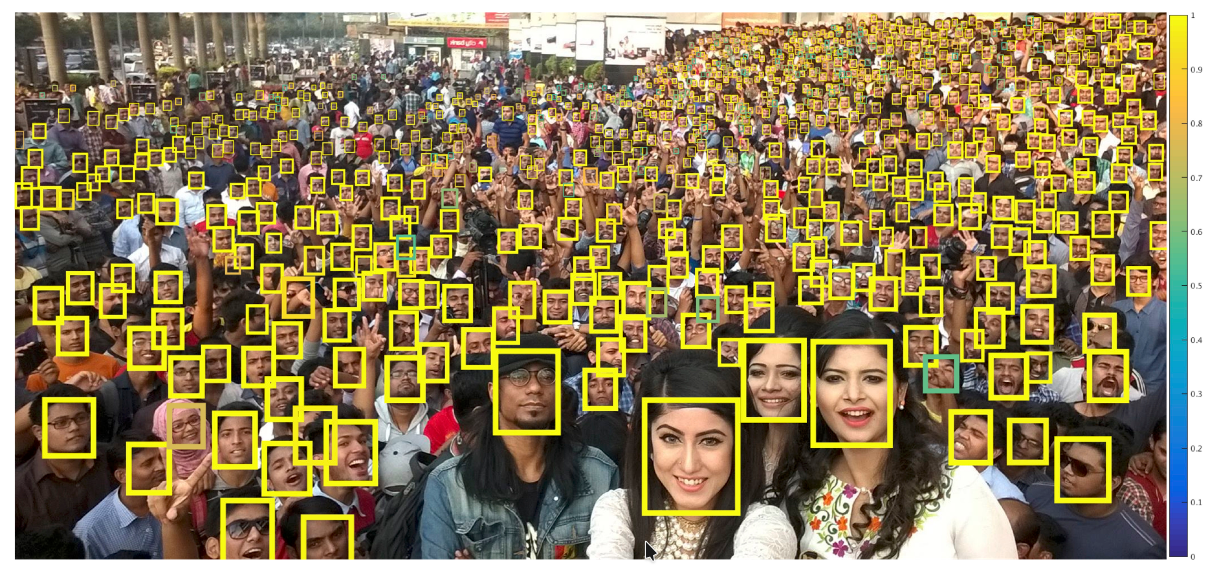
\includegraphics[width=\linewidth]{img/FindingTinyFaces.png}
\caption{Rezultati algoritma za detekciju lica iz rada \citep{findingTinyFaces}}
\label{img:findingTinyFaces}
\end{figure}

\item \textbf{Praćenje.} Ovaj pojam odnosi se na praćenje određenog objekta ili više njih u sceni. Ova kategorija se, logično, primjenjuje samo u području videa i izuzetno je bitna za sustave koji riješavaju zadatke poput autonomne vožnje.

\item \textbf{Segmentacija.} Pojam segmentacije odnosi se na proces grupiranja piksela u skupine s kojima se kasnije može raditi niz drugih procesa, npr. klasifikacija itd. 

\begin{figure}[htb]
	\centering
	\begin{subfigure}[b]{0.4\linewidth}
		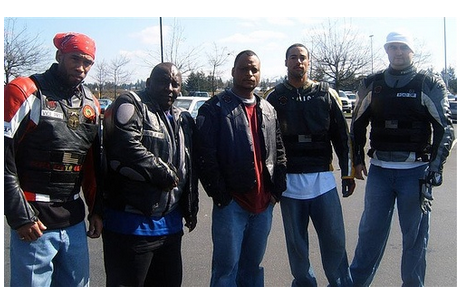
\includegraphics[width=\linewidth]{img/OriginalImage.png}
		\caption{Originalna slika}
	\end{subfigure}
	\begin{subfigure}[b]{0.4\linewidth}
		
\includegraphics[width=\linewidth]{img/ImageSegmentation.png}
		\caption{Segmentirana slika}
	\end{subfigure}
	\caption{Segmentacija slike}
	\source{NVIDIA DevBlog}
	\label{img:segmentation}
\end{figure}

Nadalje, semantička segmenatacija, kako i samo ime govori, pokušava odrediti semantičku ulogu svakog piksela u slici. Dakle, možemo reći da pokušava klasificirati svaki piksel u njegovu semantičku cjelinu. 

\begin{figure}[htb]
\centering
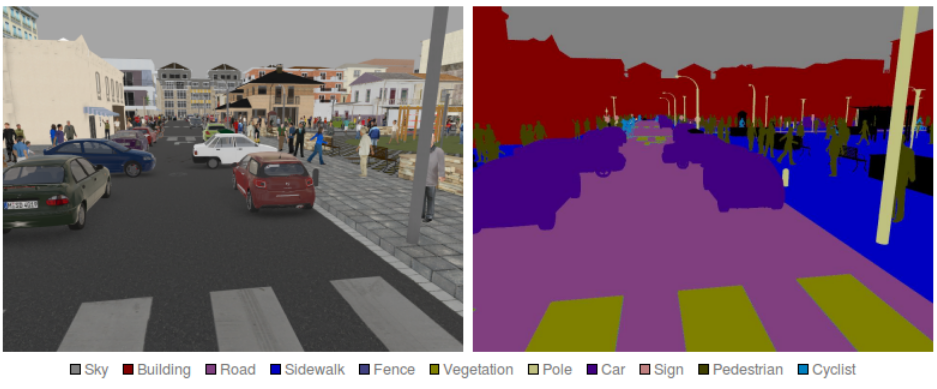
\includegraphics[width=\linewidth]{img/SemanticSegmentation.png}
\caption{Semantička segmentacija slike}
\source{NVIDIA DevBlog}
\label{img:semanticSegmentation}
\end{figure}

Instancijska segmentacija (\textit{engl.} Instance segmentation) ide i korak dalje. Ona pokušava segmentirati različite objekte istog razreda objekata. Primjerice, ako se na slici nalaze tri mobitela, svaki mobitelj bit će označen drugom bojom.

\begin{figure}[htb]
	\centering
	\begin{subfigure}[b]{0.4\linewidth}
		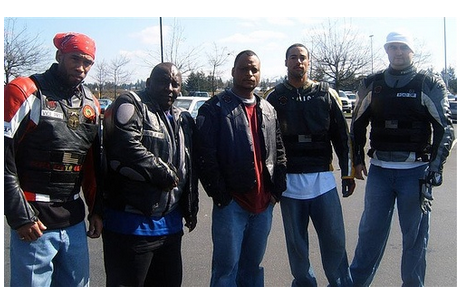
\includegraphics[width=\linewidth]{img/OriginalImage.png}
		\caption{Originalna slika}
	\end{subfigure}
	\begin{subfigure}[b]{0.4\linewidth}
		
\includegraphics[width=\linewidth]{img/InstanceSegmentation.png}
		\caption{Instancijski segmentirana slika}
	\end{subfigure}
	\caption{Instancijska segmentacija slike}
	\source{NVIDIA DevBlog}
	\label{img:instanceSegmentation}
\end{figure}

\item Ostale kategorije računalnog vida koje su manje zastupljene: Super-resolution, Style Transfer, Colourisation 

\begin{figure}[htb]
	\centering
	\begin{subfigure}[b]{0.4\linewidth}
		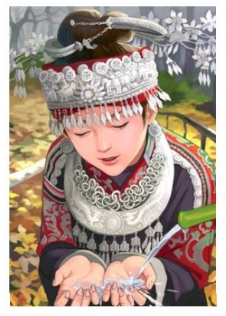
\includegraphics[width=\linewidth]{img/OriginalSRGAN.png}
		\caption{Originalna slika}
	\end{subfigure}
	\begin{subfigure}[b]{0.4\linewidth}
		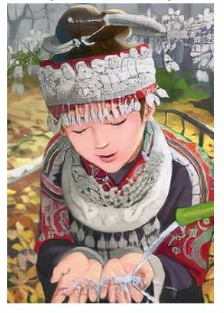
\includegraphics[width=\linewidth]{img/SRGAN.png}
		\caption{SRGAN}
	\end{subfigure}
	\caption{Slika poboljšana metodom Super-resolution GAN \citep{SRGAN}}
	\label{img:SRGAN}
\end{figure}

\begin{figure}[htb]
	\centering
	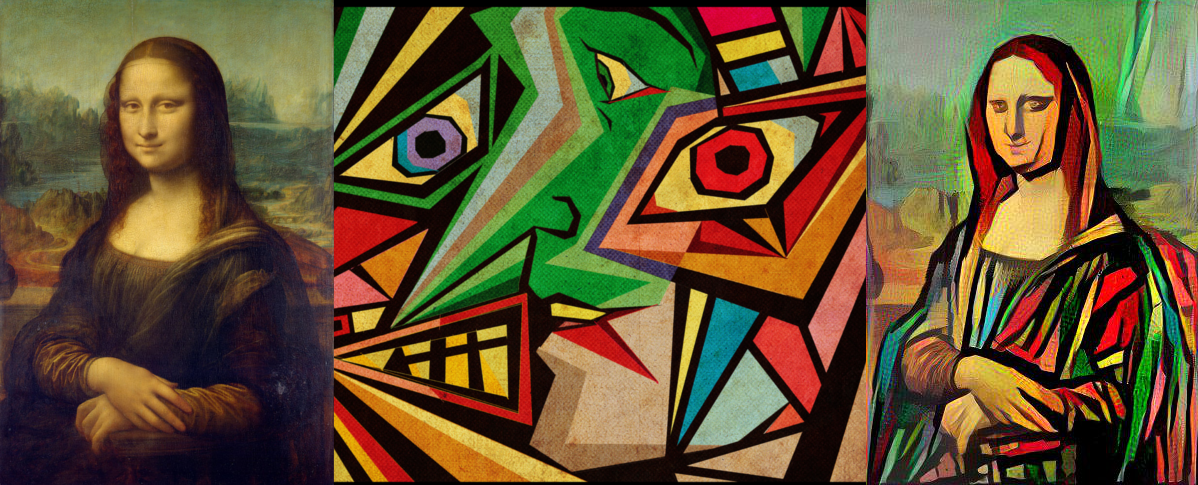
\includegraphics[width=\linewidth]{img/StyleTransfer.png}
	\caption{Prva slika prikazuje originalnu \textit{Mona Lisu}, druga slika prikazuje sliku naslikanu u stilu kubizma/ekspresionizma, treća slika prikazuje stil druge slike prenesen na prvu sliku}
	\label{img:styleTransfer}
\end{figure}

\begin{figure}[htb]
	\centering
	\begin{subfigure}[b]{0.4\linewidth}
		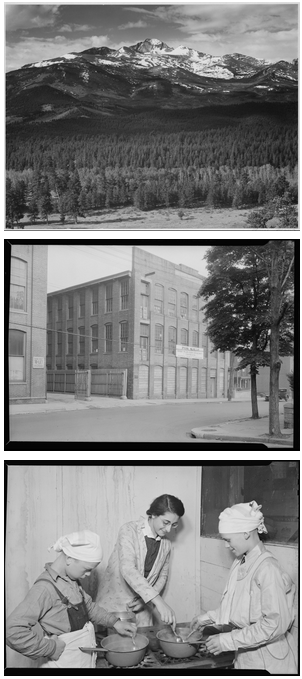
\includegraphics[width=\linewidth]{img/ColourisationOriginal.png}
		\caption{Originalna slika}
	\end{subfigure}
	\begin{subfigure}[b]{0.4\linewidth}
		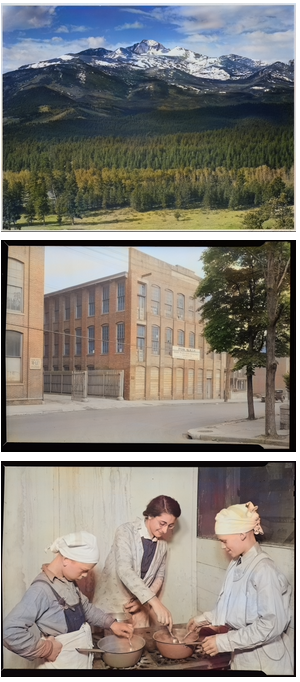
\includegraphics[width=\linewidth]{img/Colourisation.png}
		\caption{Colourisation}
	\end{subfigure}
	\caption{Slika poboljšana metodom colourisation}
	\label{img:colourisation}
\end{figure}

\end{enumerate}

